%%%%%%%%%%%%%%%%%%%%%%%%%%%%%%%%%%%%%%%%%%%%%%%%%%%%%%%%%%%%%%%%%%%%%%%%%%%%
% AGUJournalTemplate.tex: this template file is for articles formatted with LaTeX
%
% This file includes commands and instructions
% given in the order necessary to produce a final output that will
% satisfy AGU requirements, including customized APA reference formatting.
%
% You may copy this file and give it your
% article name, and enter your text.
%
%
% Step 1: Set the \documentclass
%
%

%% To submit your paper:
\documentclass[draft]{agujournal2019}
\usepackage{url} %this package should fix any errors with URLs in refs.
\usepackage{lineno}
\usepackage[inline]{trackchanges} %for better track changes. finalnew option will compile document with changes incorporated.
\usepackage{soul}
\linenumbers
\usepackage{graphicx}
\usepackage{amsmath,amsfonts,amsthm,bm}
\DeclareMathOperator{\tr}{tr}
\usepackage{amssymb}
\usepackage[fleqn,tbtags]{mathtools}
\usepackage{multirow}
\usepackage{xcolor}

\renewcommand{\Re}{\operatorname{Re} } 
\renewcommand{\Im}{\operatorname{Im} } 

\linespread{1.6}
%%%%%%%
% As of 2018 we recommend use of the TrackChanges package to mark revisions.
% The trackchanges package adds five new LaTeX commands:
%
%  \note[editor]{The note}
%  \annote[editor]{Text to annotate}{The note}
%  \add[editor]{Text to add}
%  \remove[editor]{Text to remove}
%  \change[editor]{Text to remove}{Text to add}
%
% complete documentation is here: http://trackchanges.sourceforge.net/
%%%%%%%

\draftfalse

%% Enter journal name below.
%% Choose from this list of Journals:
%
% JGR: Atmospheres
% JGR: Biogeosciences
% JGR: Earth Surface
% JGR: Oceans
% JGR: Planets
% JGR: Solid Earth
% JGR: Space Physics
% Global Biogeochemical Cycles
% Geophysical Research Letters
% Paleoceanography and Paleoclimatology
% Radio Science
% Reviews of Geophysics
% Tectonics
% Space Weather
% Water Resources Research
% Geochemistry, Geophysics, Geosystems
% Journal of Advances in Modeling Earth Systems (JAMES)
% Earth's Future
% Earth and Space Science
% Geohealth
%
% ie, \journalname{Water Resources Research}

\journalname{JGR: Solid Earth}


\begin{document}

%% ------------------------------------------------------------------------ %%
%  Title
%
% (A title should be specific, informative, and brief. Use
% abbreviations only if they are defined in the abstract. Titles that
% start with general keywords then specific terms are optimized in
% searches)
%
%% ------------------------------------------------------------------------ %%

% Example: \title{This is a test title}

\title{Impact of seondary fractures on the seismic reflectivity of large primary fractures}

%% ------------------------------------------------------------------------ %%
%
%  AUTHORS AND AFFILIATIONS
%
%% ------------------------------------------------------------------------ %%

% Authors are individuals who have significantly contributed to the
% research and preparation of the article. Group authors are allowed, if
% each author in the group is separately identified in an appendix.)

% List authors by first name or initial followed by last name and
% separated by commas. Use \affil{} to number affiliations, and
% \thanks{} for author notes.
% Additional author notes should be indicated with \thanks{} (for
% example, for current addresses).

% Example: \authors{A. B. Author\affil{1}\thanks{Current address, Antartica}, B. C. Author\affil{2,3}, and D. E.
% Author\affil{3,4}\thanks{Also funded by Monsanto.}}

\authors{Edith Sotelo\affil{1}, J. Germ\'{a}n Rubino\affil{2},  Nicol\'{a}s D. Barbosa\affil{1}, Santiago G. Solazzi\affil{1}, Klaus Holliger\affil{1}}


% \affiliation{1}{First Affiliation}
% \affiliation{2}{Second Affiliation}
% \affiliation{3}{Third Affiliation}
% \affiliation{4}{Fourth Affiliation}

 \affiliation{1}{Institute of Earth Sciences, University of Lausanne, Lausanne, Switzerland }
 \affiliation{2}{CONICET, Centro Atómico Bariloche - CNEA, San Carlos de Bariloche, Argentina}
%(repeat as many times as is necessary)

%% Corresponding Author:
% Corresponding author mailing address and e-mail address:

% (include name and email addresses of the corresponding author.  More
% than one corresponding author is allowed in this LaTeX file and for
% publication; but only one corresponding author is allowed in our
% editorial system.)

% Example: \correspondingauthor{First and Last Name}{email@address.edu}

\correspondingauthor{Edith Sotelo}{edith.sotelogamboa@unil.ch}

%% Keypoints, final entry on title page.

%  List up to three key points (at least one is required)
%  Key Points summarize the main points and conclusions of the article
%  Each must be 140 characters or fewer with no special characters or punctuation and must be complete sentences

% Example:
% \begin{keypoints}
% \item	List up to three key points (at least one is required)
% \item	Key Points summarize the main points and conclusions of the article
% \item	Each must be 140 characters or fewer with no special characters or punctuation and must be complete sentences
% \end{keypoints}

\begin{keypoints}
\item We explore poroelastic effects associated with large primary fractures connected to smaller mesoscopic secondary fractures  in predominately impermeable environments.
\item Our results show that these poroelastic effects can increase the primary fracture's normal compliance and, thus, its normal-incidence PP reflectivity.
\item Our results also show that changes in the secondary fracture properties have a variable impact on primary's fracture normal compliance and reflectivity.
\end{keypoints}

%% ------------------------------------------------------------------------ %%
%
%  ABSTRACT and PLAIN LANGUAGE SUMMARY
%
% A good Abstract will begin with a short description of the problem
% being addressed, briefly describe the new data or analyses, then
% briefly states the main conclusion(s) and how they are supported and
% uncertainties.

% The Plain Language Summary should be written for a broad audience,
% including journalists and the science-interested public, that will not have 
% a background in your field.
%
% A Plain Language Summary is required in GRL, JGR: Planets, JGR: Biogeosciences,
% JGR: Oceans, G-Cubed, Reviews of Geophysics, and JAMES.
% see http://sharingscience.agu.org/creating-plain-language-summary/)
%
%% ------------------------------------------------------------------------ %%

%% \begin{abstract} starts the second page

\begin{abstract}
Fluid pressure diffusion (FPD) between mesoscale fractures can significantly impact the seismic response of the affected rock masses. Mesoscale fractures refer to those much larger than the pore space but much smaller than the dominant wavelength. However, evidence suggest that larger macroscale fractures are the ones dominating the mechanical and hydraulic properties of the fracture network and, hence, of the fractured rock mass as a whole. We, therefore, asses the impact that FPD effects between a large macroscale primary fracture with secondary mesoscale fractures have on the  compliance and corresponding reflectivity response of the primary fracture. To this end, we consider several models, which comprise an infinite horizontal primary fracture connected to vertical mesoscale secondary fractures embedded in a background deemed impermeable at the seismic frequencies. The individual models differ only on regard to the secondary fracture properties (e.g., length, aperture and mechanical moduli, etc). We also consider a model of an isolated primary horizontal fracture for comparison.
%We then investigate the senstivity of the  primary fracture normal compliance and corresponding normal-incidence PP reflectivity due to FPD effects associated to the variations of the secondary fracture properties. 
We then perform a vertical compressional oscillatory test over samples of the aforementioned models. However, to isolate impact of FPD effects on the primary fracture, we average the vertical components of strain and stress  only over this fracture. We use these values to estimate first the corresponding P-wave modulus and then to compute the normal compliance and  PP reflectivities. Our results show that both the compliance and the PP reflectivity of the primary fracture increase as much as one and a half orders-of-magnitude. Moreover, variations in the properties of the secondary fracture influence in different degrees the aformentioned results.


\end{abstract}

%\section*{Plain Language Summary}
%Plain language summary


%% ------------------------------------------------------------------------ %%
%
%  TEXT
%
%% ------------------------------------------------------------------------ %%

%%% Suggested section heads:
% \section{Introduction}
%
% The main text should start with an introduction. Except for short
% manuscripts (such as comments and replies), the text should be divided
% into sections, each with its own heading.

% Headings should be sentence fragments and do not begin with a
% lowercase letter or number. Examples of good headings are:

% \section{Materials and Methods}
% Here is text on Materials and Methods.
%
% \subsection{A descriptive heading about methods}
% More about Methods.
%
% \section{Data} (Or section title might be a descriptive heading about data)
%
% \section{Results} (Or section title might be a descriptive heading about the
% results)
%
% \section{Conclusions}


\section{Introduction}

Fractures are ubiquitous through out the Earth's upper crust and dominate the mechanical and hydraulic propreties of the embedding rock masses \cite<e.g.,>{Jaeger2009, Liu2005}. In many cases, larger fractures intensify these effects. For instance, preferential flow is a common occurrence in fractured rock \cite{Tsang1998, Faulkner2010}, which, as simulations suggest, is further enhanced by the presence of larger fractures characterized by correlated permeabilities \cite<e.g.,>{DeDreuzy2001,Hyman2016}. These findings are supported by field evidence, which shows that high-permeability zones are dominated by large fractures, which are normally interconnected to a network of smaller fractures \cite<e.g.,>{Vidal2017, Sausse2005}. Similary, larger fractures can accentuate rock deformation. Laboratory and field measurements suggest that fracture compliance scales with fracture length \cite{Worthington2007,Hobday2012}. This implies that larger fractures tend to be more compliant and, hence, deform more readily. The numerical analysis performed by \citeA{Morris2017} supports the scaling of compliance with fracture length, although their results show that fracture compliance also depends on the current confining stress. Since large fractures tend to control the mechanical and hydraulic properties of their embedding rock masses, their characterization is of great interest in prominent applications, such as geothermal energy extraction,  CO$_2$ storage, ground water management, oil and gas explotation, nuclear waste storage, among others.

Seismic reflection methods are useful tools for fracture characterization due to the generally high reflectivity that large fractures, larger than the dominant wavelength, exhibit as a consequence of their strong mechanical constrast with the embedding background. In fact, studies show that the reflected seismic signal from a fracture plane correlates with the ratio of the fracture compliance to the seismic impedance of the background, as well as with the frequency \cite{ gu1996,Liu1995, Pyrak-Nolte1990}. 
%Thus, the more compliant fractures embedded within a comparable much stiffer background are normally associated with higher reflectivities at the seismic frequencies.
Relevant examples of seismic applications for fracture characterization are the inversion of fracture compliance from angle-dependent reflection data \cite{Cui2017, Minato2016}  as well as  the  estimation of fracture properties from the scattered wavefield generated by the spatial heterogeneities of the fracture under study \cite{Minato2014}.  However, these and similar methodologies have been largely developed within the elastic framework, which cannot account for fluid-solid interactions in the fractured rock. 

Conversely, using a poroelastic framework permits an accurate physical description of porous fractured media. The works of \citeA{Rubino2015a} and \citeA{Barbosa2017} show that poroelastic effects in fractured rock produce a frequency-dependent behavior of the normal fracture compliance. Simlarly, \citeA{Nakagawa2007} and  \citeA{Barbosa2016} demonstrate that hydraulic interactions between a poroelastic fracture and its embedding background increases the fracture reflectivity at the seismic frequencies. The described poroelastic impact on the reflectivity and the compliance of fractures is a direct consequence of fluid pressure diffusion (FPD) that takes place when seismic waves induce pressure gradients due to the mechanical contrast between the fracture and the background \cite<e.g.,>{Muller2010}. FPD increases the normal compliance of fractures as the stiffening fluid exists the fracture to equilibrate the pressure \cite{Rubino2015a, Barbosa2017}, which, in turn, leads to an increase of reflectivity. However, in many fractured environments of interest, the background is largely impermeable for the seismic frequencies, which prohibits FPD to take place with the embedding fractures. Conversely, there is far-reaching evidence indicating the pervasive presence of damage zones surrounding large fractures and faults \cite<e.g.,>{Kim2004, Faulkner2010, Savage2011}, which enhances the permeability around the fracture and, thus, provide the necessary conditions for FPD to prevail \cite{Mitchell2012, Sotelo2021}. This, consequently can produce the increase of the normal compliance of the  fracture and, thus, of its reflectivity.

Damage zones predominantly  consist of  a network of macro- and micro fractures, with a decaying density from the fault core \cite{Chester2004, Mitchell2009}. It is, therefore, likely that some of these secondary fractures are connected  to the main fault or large fracture and, thus, promote FPD , which in, turn, can induce an increase of the primary fracture reflectivity. Studies that investigate fracture-to-fracture FPD focus mainly on mesoscale fractures, which are much larger than the pore size but much smaller that the dominant wavelength. In these studies, the main objective is to investigate the effective response of the fractured rock mass regarding seismic velocities and attenuation  associated with the network properties, such as fracture density, fracture length, degree of fracture connectivity and fluid saturation, among others \cite{Rubino2014, Hunziker2018, Solazzi2020}. However, FPD effects between a large macroscale fracture, larger than the prevailing  wavelength, and secondary mesoscale fractures as well as its impact on the large fracture compliance and reflectivity response have been largely unexplored.

In this work we seek to address this issue by investigating  FPD effects between a large macroscopic primary fracture and secondary mesoscale fractures. The main goal is to evaluate the impact that this poroealstic interaction has on the primary fracture normal compliance and the corresponding PP reflectivity response at normal incidence within the seismic frequency range. To this end, we consider several models that consist of an infinite horizontal primary fracture connected to multiple vertical mesoscale fractures. We assume that this fracture system is embedded in a background deemed impermeable for the frequencies of interest (Figure \ref{fig.1}). We evaluate the sensitivity of the primary fracture compliance and its PP reflectivity to variations in the properties of the secondary fractures, such as  their lengths, spacing, mechanical moduli, among others. For comparison, we also calculate the normal compliance and reflectivity of an isolated infinite horizontal fracture. To isolate FPD effects acting only upon the primary fracture, we first perform a vertical compressional oscillatory test over samples of the aforementioned models. Then, we average the vertical components of stress and strain only over the primary fracture of interest. Using these values, we calculate the P-wave modulus and the corresponding normal compliance. Finally, we estimate the PP reflectivity at normal incidence (Figure \ref{fig.3}). For this latter, we disregard the presence of the secondary fractures since it is very unlikely that they affect the propagating P-wave, given that their fracture planes are of mesoscale size and aligned with the direction of the wave propagation.

\section{Theory and methods}
In this section, we first detail theoretical aspects regarding the validity of the frequency-dependent behavior of the P-wave modulus and corresponding normal compliance of a large primary fracture as a  consequence of FPD interactions with secondary mesoscale fractures. Then, we describe a homogenization method that permits to isolate FPD effects related only to the primary fracture to estimate its P-wave modulus and normal compliance. Finally, we outline the semi-analytical plane-wave solutions to compute the normal-incidence PP reflectivity response of the primary fracture.

\subsection{Mesoscale fluid pressure diffusion}

 \begin{figure}[!ht]
\centering
        \includegraphics[ width= 100mm, height=80mm]{fracture_system.eps}
\caption{ Schematic illustration of a fracture system composed of an infinite horizontal macroscopic primary fracture connected to equally-spaced vertical mesoscale secondary fractures embedded in a background deemed impermeable for the frequencies of interest. The light green box represents a sample $\Omega$ used to estimate the primary fracture P-wave modulus and the corresponding normal compliance of the primary fracture. The red downward arrow indicates the direction of propagation of an incoming P-wave and the black arrows inside the fracture designate the direction of the fluid flow induced by FPD.
}
\label{fig.1}
\end{figure}

We assume an incoming P-wave impinging normally onto the large primary fracture as shown  in Figure \ref{fig.1}. This produces an increment of the pore pressure in the primary fracture, which, in turn, equilibrates by inducing fluid flow towards the secondary fractures. For sufficiently low frequencies, which are in general within the seismic frequency range, this fracture-to-fracture wave-induced fluid flow is driven FPD \cite{Muller2010}.
We are interested in FPD that occurs at mesoscale heterogeneities since this is particularly relevant for seismic applications \cite{Pride2004, Muller2010}.
Mesoscale heterogeneities refer to those with characteristic length-scales  $l_h$ larger than the pore scale $l_p$ but smaller than the wavelength $\lambda_w$. For the considered fracture system, the mesoscale heterogeneities are dictated by the characteristic sizes of the fractures, for instance, the length of the secondary fractures \cite{Rubino2014} and the aperture of the primary fracture.
On the other hand, this FPD  mechanism is constrained to frequencies $f$ that are much lower than Biot's characteristic frequency $f_B$  \cite{Biot1956, Dutta1979}
\begin{linenomath*}
\begin{equation}\label{Eq.1}
f_B= \frac{1}{2 \pi} \frac{\eta \phi}{ \rho_f \kappa S },
\end{equation}
\end{linenomath*}
where $\phi$ is the porosity, $\kappa$  the static permeability, $\eta$, the fluid viscosity,  $\rho_f$ the fluid density, and $S$ the tortuosity of the pore space. The aformentioned considerations regarding frequencies and scales constraining mesoscale FPD can be summarized as
\begin{linenomath*}
\begin{equation}\label{Eq.2}
\begin{split}
f & \ll f_B\\
l_p & \ll l_h\ll \lambda_w.
\end{split}
\end{equation}
\end{linenomath*}

It can be shown that the diffusion coefficient $D$ and the characteristic diffusion $L_d$ associated with FPD are \cite{Chandler1981, Norris1993}
\begin{linenomath*}
\begin{equation}\label{Eq.3}
\begin{split}
&L_d=\sqrt{\frac{D}{\omega}},\quad \text{with} \\
&D= \frac {\kappa} {\eta} \frac{M H_d}{H},
\end{split}
\end{equation}
\end{linenomath*}
where $M$ is Biot’s fluid storage modulus, $H_d$ and $H$ are the drained and undrained plane-wave moduli, respectively, and $\omega$ is the angular frequency $\omega = 2 \pi f$.        
The required rock physical properties are calculated as
\begin{linenomath*}
\begin{equation}\label{Eq.4}
\begin{split}
& H_d = \lambda_d + 2 \mu, \\
& H = H_d + M \alpha ^2, \\
& \lambda_d= K_m - \frac{2}{3} \mu, \\
& \alpha =1-\frac{K_m}{K_s},\\
& M  =\left( \frac{\alpha-\phi}{K_s} +\frac{\phi}{K_f} \right)^{-1},
\end{split}
\end{equation}
\end{linenomath*}
where $\lambda_d$ is the the drained Lamé modulus, $\mu$ is the shear modulus, $\alpha$ is the Biot-Willis effective stress coefficient, and  $K_m$, $K_s$, and $K_f$ are the bulk moduli of the drained solid frame, the solid grains, and the pore fluid, respectively.

FPD is characterized by two limiting regimes, the relaxed and unrelaxed states, which are controlled by the frequency, the characteristic diffusion length $L_d$, and the characteristic size of the heterogeneities $l_h$ 
The relaxed state prevails at sufficiently low frequencies, for which  $L_d \gg l_h$. In this regime, there is enough time for the pressure between the main and secondary fractures to equilibrate. Conversely, the unrelaxed state prevails at sufficiently high frequencies, for which $L_d \ll l_h$ and, consequently, there is insufficient time for pressure equilibration to take place and, hence, the main and secondary fractures are hydraulically isolated. A transition zone exists at intermediate frequencies for which $L_d \approx l_h$. This transition zone is associated with attenuation and dispersion of body waves due to viscous dissipation. The maximum dissipation of energy is associated with the characteristic transition frequency $f_c= \omega_c/2\pi$, 
which depends on the diffusion coefficient $D$ and the characteristic size of the heterogeneity $l_h$ \cite{Rubino2014}
\begin{linenomath*}
\begin{equation}\label{Eq.5}
\omega_c \propto \frac{D}{(l_h)^2}.
\end{equation}
\end{linenomath*}

The described FPD relaxation mechanism produces a viscoelastic behavior of the primary fracture P-wave modulus and, consequently, of its normal compliance. 
The frequency-dependent P-wave modulus of the  primary fracture can be estimated by solving \citeauthor{Biot1941}'s \citeyear{Biot1941} on a representative sample of the fractured model of Figure \ref{fig.1}, while applying a vertical compressional oscillatory test. This is 
followed by the volume-averaging of the vertical strain and stress components, which are then used to estimate the frequency-dependent P-wave modulus.


\subsection{Homogenization procedure}
We consider a model in $\mathbb R^2$ comprised of a poroelastic fracture system embedded in a  background deemed impermeable for the frequencies of interest. The fracture system consists of an infinite primary horizontal fracture that is intersected by equally spaced vertical secondary fractures. 
(Figure \ref{fig.1}). To estimate the P-wave modulus of the primary fracture, we apply the homogenization procedure described below. This procedure is characterized by the sampling strategy suggested in the work of \citeA{Sotelo2022}, which considers a section of the poroelastic medium together with the embedding background. This sampling technique permits to naturally incorporates the boundary conditions (BC) of the embedding background, which is an important consideration when the poroelastic medium is not periodic as in this case. This sample is then subjected to a vertical compressional oscillatory test. To account for the  impact of FPD effects on the primary fracture only, the subsequent averaging of the vertical stress and strain components is performed only over the primary fracture. Finally, these averages are used to calculate the corresponding  P-wave modulus and normal compliance of the primary fracture.

Following \citeA{Sotelo2022}, we take a sample $\Omega$ of the model shown in Figure \ref{fig.1}, which consists of a representative section of the fracture system and the embedding background (Figures \ref{fig.2}). The representative section of the fracture system is composed of a portion of the poroelastic primary fracture $\Omega_{p1}$  connected to a vertical mesoscopic secondary fracture $\Omega_{p2}$. The secondary fracture is centered in the sample and the sample's width is  equal to the  spacing between the secondary fractures.

 \begin{figure}[!ht]
\centering
        \includegraphics[ width= 70mm, height=80mm]{2fracture.eps}
\caption{ Enlarged view of the sample $\Omega$ presented in Figure \ref{fig.1} consisting of a portion $\Omega_{p1}$ of the primary fracture connected to a secondary fracture $\Omega_{p2}$ and the associated section of the embedding background. $\Gamma$ is the boundary of the sample with $\Gamma = \Gamma_1^+ \cup \Gamma_1^- \cup \Gamma_3^+ \cup \Gamma_3^- $. The secondary fracture is centered in the sample and the sample has a width that is equal to the spacing between the secondary fractures.
}
\label{fig.2}
\end{figure}

\subsubsection{Governing equations}

We solve Biot's consolidation equations \cite{Biot1941} over the sample $\Omega$  for the vertical compressional oscillatory relaxation test. 
We express these equations in the solid displacement - pressure ($\bm{u}-p$) formulation in the frequency domain \cite{Quintal2011,Favino2020},  with $\bm{u} = \bm{u}(\bm{x}, \omega)$ and $p = p(\bm{x},\omega)$, where $\bm{x} \in \Omega$ is the position  and $\omega \in F$ is the angular frequency, with $F =(0,W]$. This yields
\begin{linenomath*}
\begin{equation}\label{Eq.6}
\begin{split}
& - \nabla \cdot \, \bm{\sigma} =0  \quad  \textrm{in} \quad \Omega \times F,  \\
& - i \, \alpha \nabla . \, \bm{u} -i \frac{p}{M} + \frac{1}{\omega} \,\nabla \, \cdot \, \left( \frac{\kappa}{\eta} \nabla p\right)  =0 \quad  \textrm{in} \quad \Omega \times F,
\end{split}
\end{equation}
\end{linenomath*}
where $\bm{\sigma}$ is the total stress and $i$ is the imaginary unit.

The constitutive equation relating the total stress $\bm{\sigma}$ to $\bm{u}$ and $p$ is
\begin{linenomath*}
\begin{equation}\label{Eq.7}
\begin{split}
& \bm{\sigma} =  2\mu \, \bm{\varepsilon} +  \left( \lambda_d \,  \tr( \bm{\varepsilon})\, - \alpha \,p \right) \bm{I}, \qquad \text{with}\\
& \bm{\varepsilon} = \frac{1}{2} \left( \nabla \,\bm{u} + ({\nabla  \bm{u}})^T  \right),
\end{split}
\end{equation}
\end{linenomath*}
where $\bm{\varepsilon}$ is the strain tensor and $\bm{I}$ the identity tensor. 


\subsubsection{Vertical compressional oscillatory relaxation test}
In this subsection, we detail the BC for the vertical oscillatory relaxation test. We assume a Cartesian coordinate system in $\mathbb R^2$ with the associated basis vectors $\bm{\hat x_1}$ and $\bm{\hat x_3}$ parallel to the horizontal and vertical Cartesian axes, respectively. We also
let the sample $\Omega$ be a quadrilateral with boundary $\Gamma = \Gamma_1^+ \cup \Gamma_1^- \cup \Gamma_3^+ \cup \Gamma_3^- $, where $\Gamma_1^+ $ and $\Gamma_1^- $ are opposite boundaries with outer normal vectors $\bm{\hat x_1}$ and $ -\bm{\hat x_1}$, respectively. Similarly, $\Gamma_3^+ $ and $\Gamma_3^- $ are opposite boundaries with outer normal vectors $\bm{\hat x_3}$ and $ -\bm{\hat x_3}$ (Figure \ref{fig.2}). To simplify the notation, we let $ \bm{\hat n}$ be the outer normal vector
of $\Gamma$.

In the following, we define the BC for displacements, pressure, tractions and fluid flux relative to the solid, imposing periodicity to the respective variables on opposite boundaries. 
The BC for displacements are

\begin{linenomath*}
\begin{equation}\label{Eq.8}
\begin{split}
&  \bm{u} \cdot \bm{\hat{x}_3} \, \vert_{\Gamma_3^-} - \bm{u}\cdot \bm{\hat{x}_3}\, \vert_{\Gamma_3^+} =- \Delta u, \\
&  \bm{u} \cdot \bm{\hat{x}_1}\, \vert_{\Gamma_3^-} - \bm{u} \cdot \bm{\hat{x}_1} \, \vert_{\Gamma_3^+} = 0, \\
& \bm{u}\,\vert_{\Gamma_1^+} - \bm{u}\,\vert_{\Gamma_1^-} = \bm{0},
\end{split}
\end{equation}
\end{linenomath*}
where $\Delta u$ is a real displacement difference in the frequency domain.

The respective BC for pressure, tractions and fluid flux relative to the solid are
\begin{linenomath*}
\begin{equation}\label{Eq.9}
\begin{split}
& p\vert_{\Gamma_k^+}-p\vert_{\Gamma_k^-} =0, \\
& \left(\bm{\sigma}\cdot \bm{\hat n} \right)\, \vert_{\Gamma_k^+}-\left(\bm{\sigma}\cdot \bm{\hat n} \right)\, \vert_{\Gamma_k^-} = \bm{0},\\
&\left( \frac{\kappa}{\eta} \nabla p \cdot \bm{\hat n} \right) \, \vert_{\Gamma_k^+} -\left( \frac{\kappa}{\eta} \nabla p \cdot \bm{\hat n} \right) \, \vert_{\Gamma_k^-} = 0,
\end{split}
\end{equation}
\end{linenomath*}
where the subscript $k$ in $\Gamma_k^-$ and $\Gamma_k^+$ takes the value of 1 or 3 at a time to denote opposite boundaries.

\subsubsection{Plane-wave modulus}

Here, we detail the calculations to obtain the plane-wave modulus and normal compliance of the main horizontal fracture.  To this end, we first take the average of the stress component $\langle \sigma_{33} \rangle_{\Omega_{p1}}$ and of the respective strain component $\langle \varepsilon_{33} \rangle_{\Omega_{p1}}$ only over $\Omega_{p1}$ (Figure \ref{fig.2}). The corresponding average quantities $\langle \Box \rangle_{\Omega_{p1}}$ are computed as
\begin{linenomath*}
\begin{equation}\label{Eq.10}
\begin{split}
&\langle \Box \rangle_{\Omega_{p1}} = \frac{1}{\vert \Omega_{p1} \vert} \int_{\Omega_{p1}} \Box \, d\Omega_{p1}, \qquad \text{with} \quad  \vert \Omega_{p1} \vert = \int_{\Omega_{p1}}  d\Omega_{p1}.
\end{split}
\end{equation}
\end{linenomath*}

Then, we calculate the complex and frequency-dependent P-wave plane modulus $H(\omega)$ of the primary fracture as
\begin{linenomath*}
\begin{equation}\label{Eq.11}
H(\omega)= \frac{\langle \sigma_{33} \rangle_{\Omega_{p1}}}{\langle \varepsilon_{33} \rangle_{\Omega_{p1}}}.
\end{equation}
\end{linenomath*} 

Finally, we obtain the complex and frequency-dependent normal compliance $Z_N (\omega) $ of the primary fracture as
\begin{linenomath*}
\begin{equation}\label{Eq.12}
Z_N(\omega)= \frac{a_f}{H(\omega)}, 
\end{equation}
\end{linenomath*} 
where $a_f$ is the aperture of the primary fracture. 

The maximum magnitude of the imaginary part of the normal compliance ($ |\Im(Z_N (\omega))|$) is associated with maximum energy dissipation \cite{Rubino2015a} that occurs in the transition regime of FPD. Consequently, it can be used to estimate the characteristic transition frequency $f_c$, that is, to find the frequency which maximizes $ |\Im(Z_N (\omega))|$.


\subsection{P-wave normal reflectivity of the primary fracture}
We consider a simplified  model in $\mathbb R^1$ as shown in Figure \ref{fig.3}. In this model, the primary fracture is represented by a viscoelastic layer $\Omega_v$ characterized by the frequency-dependent P-wave modulus calculated applying the previously described homogenization procedure. This fracture is embedded in the half-spaces $\Lambda_1$ and $\Lambda_2$ (Figure \ref{fig.3}), which have the same rock properties as the embedding background of Figure \ref{fig.1}. In summary, we have further idealized the initial model presented in Figure \ref{fig.1} to that one shown in  Figure \ref{fig.3}, which disregards the presence of the secondary fractures. This is possible because we consider a P-wave propagating normally to the plane of the primary fracture. Under this scenario, the propagating wave will mostly be affected by changes in the P-wave modulus of the primary fracture due to the FPD interactions with the secondary fractures. Conversely,, the secondary fractures are unlikely to affect the P-wave propagation not only because their planes are parallel to the direction of the propagation but also because their sizes are very small compared to the dominant wavelength. As stated before, we  assume an incoming P-wave impinging normally on the interface $\Pi_1$ between the upper half-space and the viscoelastic fracture (Figure \ref{fig.3}). In the following, we detail the procedure to find the corresponding PP reflection coefficients at this interface.

 \begin{figure}[!ht]
\centering
        \includegraphics[ width= 80mm, height=80mm]{mainfracture.eps}
\caption{ Simplified 1-D model of that one shown in Figure \ref{fig.1}. For this case the primary fracture $\Omega_v$ is represented by a viscoelastic thin layer characterized by a frequency-dependent P-wave modulus and the secondary fractures are disregarded. The embedding background is represented by the  elastic half-spaces $\Lambda_1$ and $\Lambda_2$ with the same rock physical properties as those considered for the embedding background in Figure \ref{fig.1}. We 
use this model to compute the PP reflectivities at normal incidence at the the interface $\Pi_1$ between the primary fracture $\Omega_v$ and the upper half-space $\Lambda_1$. The downward arrow represents the incoming P-wave, while the upward arrow designates the reflected P-wave.
}
\label{fig.3}
\end{figure}

\subsubsection{Governing equations}
We formulate the elastic and viscoelastic wave equations in the space-frequency domain. For the elastic wave equation, we let $\bm{u}^e=\bm{u}^e (\bm{x},\omega)$ be the displacement vector for any position $\bm{x}$ $\in n$, with  $n= \{\Lambda_1, \Lambda_2\} $ and angular frequency  $\omega \in F$ , with $F =(0,W]$. We also let $\bm{\sigma}^e$ be the stress tensor field acting upon the medium. Then, we express the corresponding equation of motion as
\begin{linenomath*}
\begin{equation}\label{Eq.13}
- \, \rho_b \,\omega^2 \, \bm{u}^e = \nabla . \, \bm{\sigma}^e \quad  \textrm{in} \quad n \times F.
\end{equation}
\end{linenomath*}
The associated constitutive equation is given by: 
\begin{linenomath*}
\begin{equation}\label{Eq.14}
\bm{\sigma}^e = \mu \,  \left( \nabla \, \bm{u}^e + ({\nabla  \bm{u}^e})^T  \right) + \lambda \,  \nabla . \, \bm{u}^e\,\, \bm{I},
\end{equation}
\end{linenomath*}
where $\lambda$ is the undrained Lamé modulus and is calculated as $\lambda = \lambda_d + M \alpha^2$.

For the viscoelastic wave equation, we let $\bm{u}^v=\bm{u}^v (\bm{x},\omega)$ be the displacement vector for any position $\bm{x}$  $ \in \Omega_v$ and angular frequency $\omega \in F$ , with $F =(0,W]$. We also let $\bm{\sigma}^v$ be the stress tensor acting upon the medium. Then, we express the corresponding equation of motion as
\begin{linenomath*}
\begin{equation}\label{Eq.15}
- \, \rho_b \,\omega \, \bm{u}^v = \nabla . \, \bm{\sigma}^v \quad \textrm{in} \quad \Omega_v \times F.
\end{equation}
\end{linenomath*}
The associated constitutive equation is given by
\begin{linenomath*}
\begin{equation}\label{Eq.16}
\begin{split}
& \bm{\sigma}^v = \mu \,  \left( \nabla \, \bm{u}^v + ({\nabla  \bm{u}^v})^T  \right) + \lambda(\omega) \,  \nabla . \, \bm{u}^v\,\, \bm{I}, \quad \text{with} \\
& \lambda(\omega)= H(\omega)-2\mu.
\end{split}
\end{equation}
\end{linenomath*}

\subsubsection{Solution for displacements}
As stated above, we consider an incoming P-wave strikes normally the interface $\Pi_1$  between the upper half-space and the fracture (Figure \ref{fig.3}). The half-spaces and the fracture are represented by elastic and viscoelastic media, respectively. As a consequence, only P-waves propagate vertically in both half-spaces and in the fracture. Then, to find the total displacement in each medium, we sum the corresponding upgoing and downgoing P-waves, respectively.

For the elastic half-spaces $n =\{\Lambda_2, \Lambda_2\}$, we let $u_n^e$ be the corresponding total displacements, which are calculated as
\begin{linenomath*}
\begin{equation}\label{Eq.17}
\begin{split}
& u_n^e=  u_{n\,{D_P}}^e + u_{n\,{U_P}}^e \quad \text{when}\, n=\Lambda_1 , \, \text{or}  \\
& u_n^e = u_{n\,{D_P}}^e \quad \text{when}\, n=\Lambda_2 ,
\end{split}
\end{equation}
\end{linenomath*}
where $D$ and $U$ refer to the downgoing and upgoing waves, respectively, and the subscript $P$ refers to the P-wave.
% Since in the lower half-space $\Lambda_2$ there are no upgoing P-wave, $u_n^e$ simplifies to:
%\begin{linenomath*}
%\begin{equation}\label{Eq.18}
%u_n^e = u_{n\,{D_P}}^e.
%\end{equation}
%\end{linenomath*}

Then, we express the corresponding solution $u_{n\,j}^e$ for each elastic medium $n$ = $\Lambda_1$ and $\Lambda_2$, with $j$ = $D_P$ or $U_P$, as
\begin{linenomath*}
\begin{equation}\label{Eq.18}
u_{n\,j}^e = E_{n \,j} \;\exp[ \pm\; i \; k_{n}^e \; x_3 ]\,,
\end{equation}
\end{linenomath*}
where $E_{n \,j}$ is the amplitude of the corresponding elastic displacement and $x_3$ is the position. Negative and positive signs in the exponential correspond to downgoing and upgoing waves, respectively, $ k_{n}^e$ is the elastic scalar wavenumber for the P-wave in medium $n$, calculated as $ k_{n}^e$ = $\omega / V_P^n$, where $V_P^n$ is the P-wave velocity of medium $n$, with $V_P^n = \sqrt{(\lambda^n +  2\, \mu^n)/\rho_b^n}$
%The corresponding $V_P^n$ is
%\begin{linenomath*}
%\begin{equation}\label{Eq.20}
%V_P^n = \sqrt{\frac{\lambda^n +  2\, \mu^n}{\rho_b^n}}.
%\end{equation}
%\end{linenomath*}

For the viscoelastic medium $\Omega_v$, we let  $u^v$ be the total viscoelastic displacement given by 
\begin{linenomath*}
\begin{equation}\label{Eq.19}
u^v=  u_{\,D_P}^v  + u_{\,U_P}^v.
\end{equation}
\end{linenomath*}

Then, we express the solution of the corresponding displacement $u_j^v$, with $j = D_P , U_P$ as
\begin{linenomath*}
\begin{equation}\label{Eq.20}
u_j^v = V_j \;\exp[ \pm\; i \; k^v \; x_3 ]\,,
\end{equation}
\end{linenomath*}
where $V_j$ is the amplitude of the corresponding viscoelastic displacement, $ k^v$ is the viscoelastic scalar wavenumber for the P-wave calculated as $ k^v=\omega / V_P(\omega)$, where $V_P(\omega)$ is the frequency-dependent P-wave velocity that is computed as $V_P(\omega) = \sqrt{H(\omega) /\rho_b }$
%\begin{linenomath*}
%\begin{equation}\label{Eq.23}
%V_P(\omega) = \sqrt{ \frac{H(\omega) }{\rho_b} }.
%\end{equation}
%\end{linenomath*}

\subsubsection{PP reflection coefficients}
If we assume that the amplitude of the incident P-wave is one, then the reflection coefficient $R_{PP}$ at the upper half-space is equal to $E_{\Lambda_1\, UP}$ (Equation \eqref{Eq.18}). To solve for the unknown amplitudes,  we assemble a set of equations by imposing continuity of displacements and tractions at the elastic-viscoelastic interfaces $\Pi_q$, respectively, with $q=1,2$
\begin{linenomath*}
\begin{equation}\label{Eq.21}
\begin{split}
&  \left. \left(  u_n^e -  u^v \right) \right \rvert_{\Pi_q} = 0 \,, \\
&  \left. \left( t_n^e  - t^v  \right) \right \rvert_{\Pi_q} = 0 \,.
\end{split}
\end{equation}
\end{linenomath*}
Here, $n$ = $\Lambda_q$, $t_n^e$ and $t^v$ are the normal traction components on the elastic and viscoelastic sides of the interface, respectively. They are calculated as $t_n^e =( \bm{\sigma_n}^e \cdot \bm{\hat {x}_3})\cdot \bm{\hat {x}_3} $ and  
$t^v =( \bm{\sigma}^v \cdot \bm{\hat {x}_3})\cdot \bm{\hat {x}_3} $, respectively.

\section{Results}

In the following, we present a sensitivity analysis where we vary the geometrical and physical properties of the secondary fractures to investigate their impact on the normal compliance and reflectivity of the primary fracture. 
We compare the  results against those obtained using a model that considers an isolated  primary fracture embedded in impermeable background. As described below, the normal compliance of this fracture is the so-called undrained normal compliance. Similarly, its reflectivity is calculated applying the procedure described in the Theory and Methods section but, for this case, we replace the frequency-dependent plane-wave modulus $H(\omega)$ by its undrained plane-wave modulus $H$ (Equation \eqref{Eq.4}). 

Table \ref{table.1} shows the rock physical reference properties for the primary fracture, secondary fractures and the impermeable half-spaces, respectively. Table \ref{table.2} lists the properties of the pore fluids considered.
Unless stated otherwise, we assume that the pores of all fractures are water-saturated. We remark that for the elastic background, its grain and frame bulk moduli are equal. This yields a Biot- Willlis effective stress coefficient $\alpha$ equal to zero. Meaning that, the pore fluid pressure does not have any effect on the total stress and on the volumetric deformation of the solid (Equations \eqref{Eq.6} and \eqref{Eq.7}). Moreover, the background permeability is so low (1.e-12 D) that for the seismic frequencies it behaves as an impermeable medium. In summary, due to its assigned properties, the background behaves effectively as an elastic medium.
To obtain both the frequency-dependent P-wave modulus and normal compliance of the primary fracture for the different tested models,  we apply the homogenization procedure described in the Methodology section using a square sample $\Omega$ (Figure \ref{fig.2}) with a side length of 3.2 m. This homogenization procedure is valid for frequencies that are much lower than Biot's characteristic frequency (Equation \eqref{Eq.1}). The corresponding values for the primary and secondary fractures are 103.2 Hz and 116.1 Hz respectively, which are at the high end of the standard exploration seismic frequency range. Although the upper limit of the seismic band is, for practical purposes, within the same order-of-magnitude of the computed Biot's characteristic frequencies, we can still consider that the results obtained under the FPD assumption are valid. This is because a smooth transition is expected from the FPD mechanism characterized by viscous-dominated solid-fluid drag forces towards a wave induced fluid-flow mechanism controlled by an inertia-dominated drag \cite{Rubino2014}. Thus, the results we present in the following are considered valid for frequencies up to $\sim$ 100 Hz.

\begin{table}[!ht]
  \caption{Reference values of the physical properties for the primary fracture, secondary fractures, and the background, respectively (Figure \ref{fig.1}). }
\begin{center}
  \begin{tabular}{ | l c  c  c | }
    \hline
    Property & primary fracture ($f$) & Secondary fracture ($h$) & Background rock \\ \hline
    Grain bulk modulus $K_s$ (GPa) & 37 & 37 & 37 \\ 
    Porosity $\phi$ & 0.8 & 0.9 & 0.015 \\ 
    Frame bulk modulus $K_m$ (GPa) &  0.004 & 0.008 & 37\\ 
    Frame shear modulus $\mu$ (GPa) & 0.002 & 0.004 & 29\\
    Permeability $\kappa$ (D) & 1250 & 1250 & 1.e-12\\
    Aperture $a$ (m) & 0.001 & 0.001 & NA\\
    Length $L$ (m) & infinite & 3.04 & NA \\
    Spacing $s$ (m) & NA & 3.2
     & NA \\
    Grain density $\rho_s$ ($\rm{Kg/m^3}$) & 2730 & NA & 2730\\ 
    \hline
  \end{tabular}
  \label{table.1}
\end{center}
\end{table}

\begin{table}[!ht]
  \caption{Reference values of the physical properties of pore fluids}
\begin{center}
  \begin{tabular}{ | l  c  c |  }
    \hline
    Property & Water & Gas\\ \hline
    Fluid density $\rho_f$ ($\rm{Kg/m^3}$) & 1000 & 78\\
    Fluid bulk modulus $K_f$ (\rm{GPa}) & 2.25 & 0.012\\
    Fluid viscosity $\eta$ (\rm{Pa.s})& 1.e-3 & 1.5e-4\\
    \hline
  \end{tabular}
  \label{table.2}
\end{center}
\end{table}

In the following, we present plots of the frequency-dependent fracture normal compliance $Z_N (\omega)$ as a ratio against its undrained value $Z^u_{N}$, that is $Z_N\,\text{ratio} =Z_N (\omega)/ Z^u_{N}$, where the undrained normal compliance  $Z^u_{N}$ designates the minimum theoretical value $Z_N (\omega)$ can take, which corresponds to its unrelaxed state. This is calculated as $Z^u_{N}= a_f/H$. Using the properties for the primary fracture from Table \ref{table.1}, we  find that $Z^u_{N} =3.6 \times 10 ^{-13}$  m/Pa. Conversely, the drained normal compliance $Z^d_{N}$ denotes maximum thoeretical value that $Z_N (\omega)$ can take if it were possible to drain all the pore fluid from the primary fracture. This is calculated as
$Z^d_{N}= a_f/H_d$. Using again the properties for the primary fracture from Table \ref{table.1}, we find  $Z^d_{N} =1.5\times 10^{-10} $ m/Pa. However, it is expected that the magnitude of the relaxed $Z_N(\omega)$ is lower than the drained one since the secondary fractures provide a limited pore volume to drain the fluid from the primary fracture.
Finally, the theoretical maximum $Z_N$ ratio happens when  $Z_N (\omega) = Z^d_{N} $, which yields $Z^d_{N}/Z^u_{N}$ = 416.5. 
%Besides,
%we estimate the associated characteristic frequency $f_c$ by finding the frequency for which the magnitude of the imaginary part of the primary fracture compliance reaches it maximum.


\subsection{Sensitivity to the geometrical properties of the secondary fractures}
In this subsection, we investigate the sensitivity of the primary fracture normal compliance and of its reflectivy response to variations in the geometrical properties of the secondary fractures, such as length $L^h$, aperture $a^h $, and spacing $s^h$. To perform this sensitivity analysis, we modify one parameter at a time by halving repeatedly its value to a maximum of 8-fold decrement with regard to its reference value (Table \ref{table.1}).

Figure \ref{fig.4} presents the $Z_N$ ratio as a function of frequency for the different geometrical parameters of the secondary fractures. The results show that there is an increase of the normal compliance of the primary fracture with respect to its unrelaxed value ($Z_N$ ratio of 1) for all tested parameters of the secondary fractures. This is the consequence of FPD with the secondary fractures prevailing in regimes other than the unrelaxed one. Specifically, at sufficiently low frequencies, the
$Z_N$ ratio shows a constant maximum as the result of FPD occurring in the relaxed regime. Consequently, we denote this $Z_N$ ratio as the relaxed one. We remark that, the theoretical upper limit of the relaxed $Z_N$ ratio is the one associated with the drained compliance of the primary fracture, which, as previously mentioned, is equal to 416.5. 
Then, as frequency increases, the transitional FPD regime prevails, which induces the monotonic decrease of the $Z_N$ ratio towards its unrelaxed value. The results show that the relaxed $Z_N$ ratio increases with increasing magnitudes of the length $L^h$ and aperture $a^h$ of the secondary fractures and with decreasing  values of their spacing $s^h$.
Nonetheless, the sensitivity of the $Z_N$ ratio to these different geometrical properties is nuanced.
The relaxed $Z_N$ ratio is the most sensitive to variations in the length $L^h$ of secondary fractures (Figure \ref{fig.4}a) and is the least sensitive to variations in their spacing $s^h$ (Figure \ref{fig.4}c). An intermediate sensitivity is associated to variations in their aperture $a^h$ (Figure \ref{fig.4}b). Specifically, the relaxed $Z_N$ ratio shows an increase of $\sim$ 13-fold, from  3.3 to 43.5, for the corresponding 8-fold increase in length $L^h$. Then, the relaxed $Z_N$ ratio increases close to 3-fold, from 15.0 to 43.5, for a similar 8-fold aperture $a^h$ increase. Finally, the relaxed $Z_N$ ratio presents the lowest increase of $\sim$ 1.5-fold, from 43.5 to 71.2, in response to the 8-fold decrease in spacing $s^h$. 

Overall, these results show that longer secondary fractures cause  higher pressure gradients and provide progressively greater pore volumes for FPD to occur with the primary fracture. This process, then, generates a sensible increase of the normal compliance of the primary fracture as  larger volumes of its stiffening fluid flows towards the secondary fractures. Conversely, although the changes in aperture of the secondary fractures reflect the same pore volume variations as those produced by the changes in length, their impact on the sensitivity of the primary fracture normal compliance is less pronounced. This observation can be explained by the lower pressure gradients that variations in aperture produce compared to similar variations in fracture length. This is turn, results in a lower normal compliance of the primary fracture as less of its fluid flows towards the secondary fractures. Variations in the spacing of the secondary fractures  result in a similar effect to that of changes in aperture on the sensitivity of the normal compliance of the primary fracture.  As explained, this can be the result of lower pressure gradients that decreasing values of spacing produce, despite of the increasing pore volume that this creates.

On the other hand, the considered properties of the secondary fractures influence differently the characteristic transition frequency $f_c$ of the primary fracture normal compliance . For instance, $f_c$ presents the highest sensitivity to changes in length $L^h$ of the secondary fractures (Figure \ref{fig.4}a), showing decreasing values from $\sim$ 1.0 kHz to $\sim$ 5.6 Hz as the length $L^h$ increases. In contrast, $f_c$ is the least sensitive to changes in the aperture $a^h$ of the secondary fractures (Figure \ref{fig.4}b). In this case $f_c$, takes increasing values from  $\sim$ 4.0 Hz to  $\sim$ 5.6 Hz as the aperture $a^h$ increases. Finally, $f_c$ presents an intermediate sensitivity to the spacing $s^h$ of the secondary fractures (Figure \ref{fig.4}c), where it decreases from  $\sim$ 44.6 Hz to  $\sim$ 5.6 Hz with increasing spacing.

Next, the increase in normal compliance of the primary fracture as a consequence of FPD effects with the secondary fractures also have a strong impact on the primary fracture PP reflectivity. Figure \ref{fig.5} presents the absolute value of normal-incidence PP reflectivities of the primary fracture as a function of frequency for the same geometrical parameters of the secondary fractures presented in Figure \ref{fig.4}.
% We observe that for all the cases tested, the PP reflectivity of the primary fracture increases from its elastic value as a consequence of FPD occurring between the main and secondary fractures.
The results show that, for sufficiently low frequencies, the reflectivity of the primary fracture presents a maximum increase from the elastic reference as a consequence of FPD towards the secondary fractures prevailing in the relaxed regime. However, for increasingly higher frequencies, the primary fracture reflectivity  decreases monotonically towards its elastic limit, which is the result of FPD transitioning towards its unrelaxed state. Regarding the primary fracture reflectivity in the relaxed FPD regime, the highest reflectivity increase of $\sim$ 65-fold is associated with most closely spaced secondary fractures ($s^h$ = 0.4 m in Figure \ref{fig.5}c). Similarly, the second largest increase in reflectivity of $\sim$ 44-fold corresponds to both the largest ($L^h$ = 3.04 m in Figure \ref{fig.5}a) and the widest ($a^h$ = 0.001 m in Figure \ref{fig.5}c) secondary fractures.
Regarding the sensitivity of the primary fracture reflectivity to changes in the geometrical properties of the secondary fractures, the results show that it presents a similar behavior as the one described for its normal compliance. 
That is, its reflectivity at normal incidence is the most sensitive to changes in length $L^h$, then aperture $a^h$, and, finally, spacing $s^h$. 
%Specifically, the maximum increase of reflectivity is around two orders of magnitude for an eight-fold increment in the length $L^h$ However, For a similar eight-fold increase in aperture $a^h$, from 0.125 mm to 1 mm, the maximum increase of the corresponding reflectivity is only around one order of magnitude. Finally the maximum increase of reflectivity is within the same order of magnitude for an eight-fold decrease in spacing $s^h$.

 \begin{figure}[!ht]
\centering
        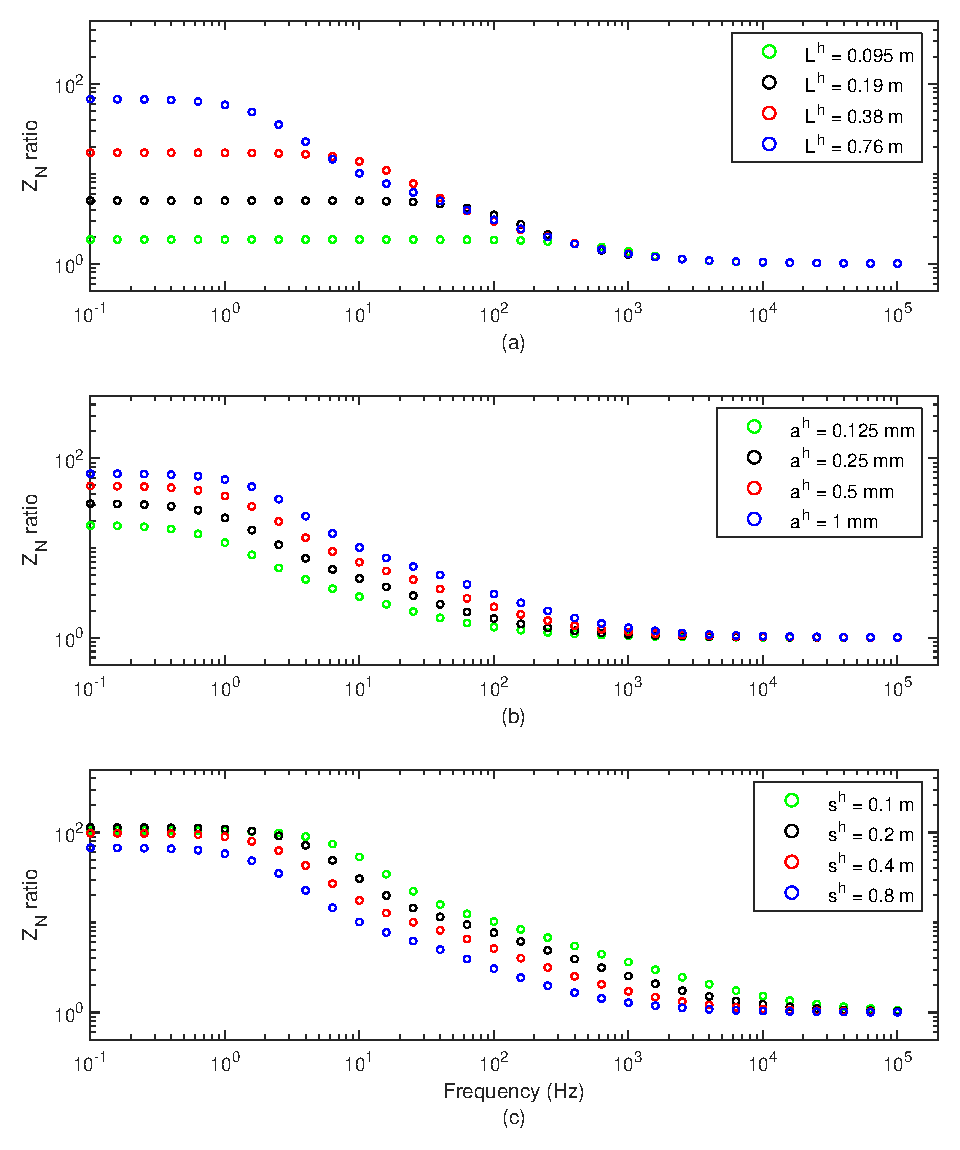
\includegraphics[ width=110mm, height=120mm]{sensitivityZN_geometry.eps}
\caption{Ratio of the frequency-dependent normal fracture compliance to its undrained normal compliance ($Z_N\, \text{ratio}$) as a function of frequency obtained considering secondary fractures presenting different a) lengths $L^h$, b) apertures $a^h$ and  c) spacings $s^h$.
}
\label{fig.4}
\end{figure}

 \begin{figure}[!ht]
\centering
        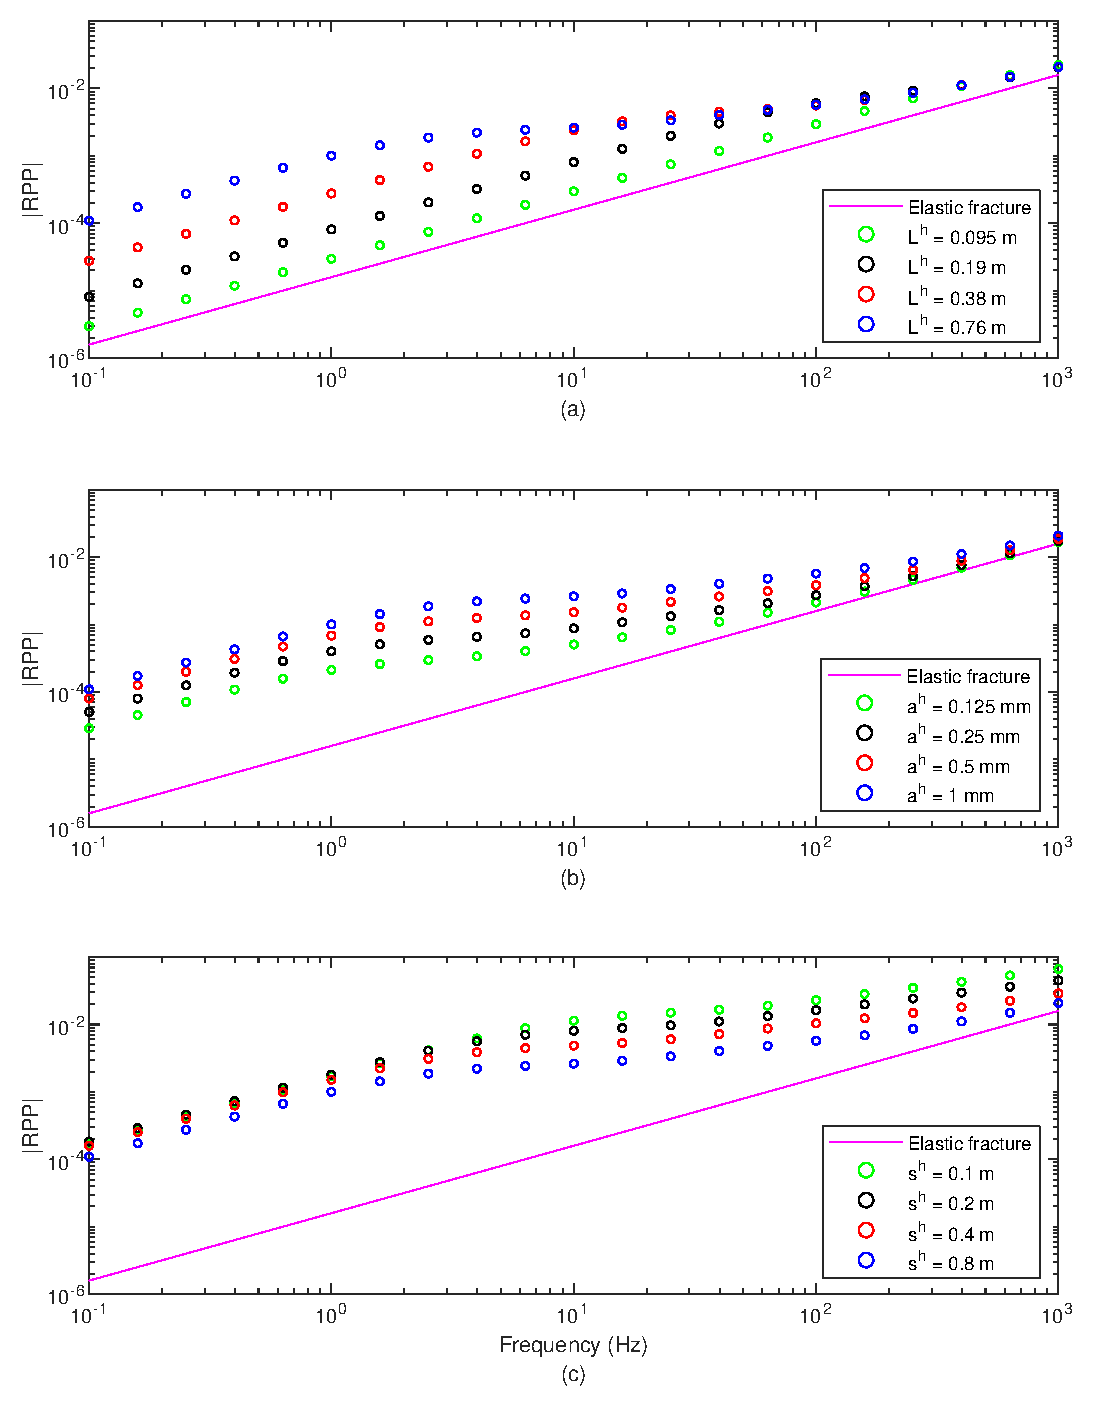
\includegraphics[ width=100mm, height=120mm]{sensitivityRPP_geometry.eps}
\caption{ Absolute value of normal-incidence P-wave reflection coefficients as a function of frequency obtained considering different frequency-dependent P-wave moduli of the primary fracture. These moduli include the effect of FPD interactions with secondary fractures presenting different a) lengths $L^h$, b) apertures $a^h$ and  c) spacings $s^h$. For comparison,  we also show the reflectivity of an isolated, that is, elastic primary fracture.
}
\label{fig.5}
\end{figure}



\subsection{Sensitivity to the physical properties of the secondary fractures}
In this subsection, we investigate the sensitivity of the primary fracture normal compliance and of its reflectivy response to variations in the physical  properties of the secondary fractures, such as their bulk $K_m^h$ and shear $\mu^h$ moduli, permeability $\kappa^h $ and pore fluid type $f^h$, respectively. To perform this sensitivity analysis, we again modify one parameter at a time, taking as the reference values the ones specified in Table \ref{table.1}. For the mechanical moduli, we repeatedly double the bulk modulus $K_m^h$, keeping the ratio $K_m^h/ \mu^h =2$. To investigate the sensitivity to the permeability $\kappa^h$, we repeatedly decrease its value by 50\%. Finally, to study the sensitivity to the pore fluid $f^h$, we compare the results of considering water and gas as saturating fluids in the secondary fractures.

 \begin{figure}[!ht]
\centering
        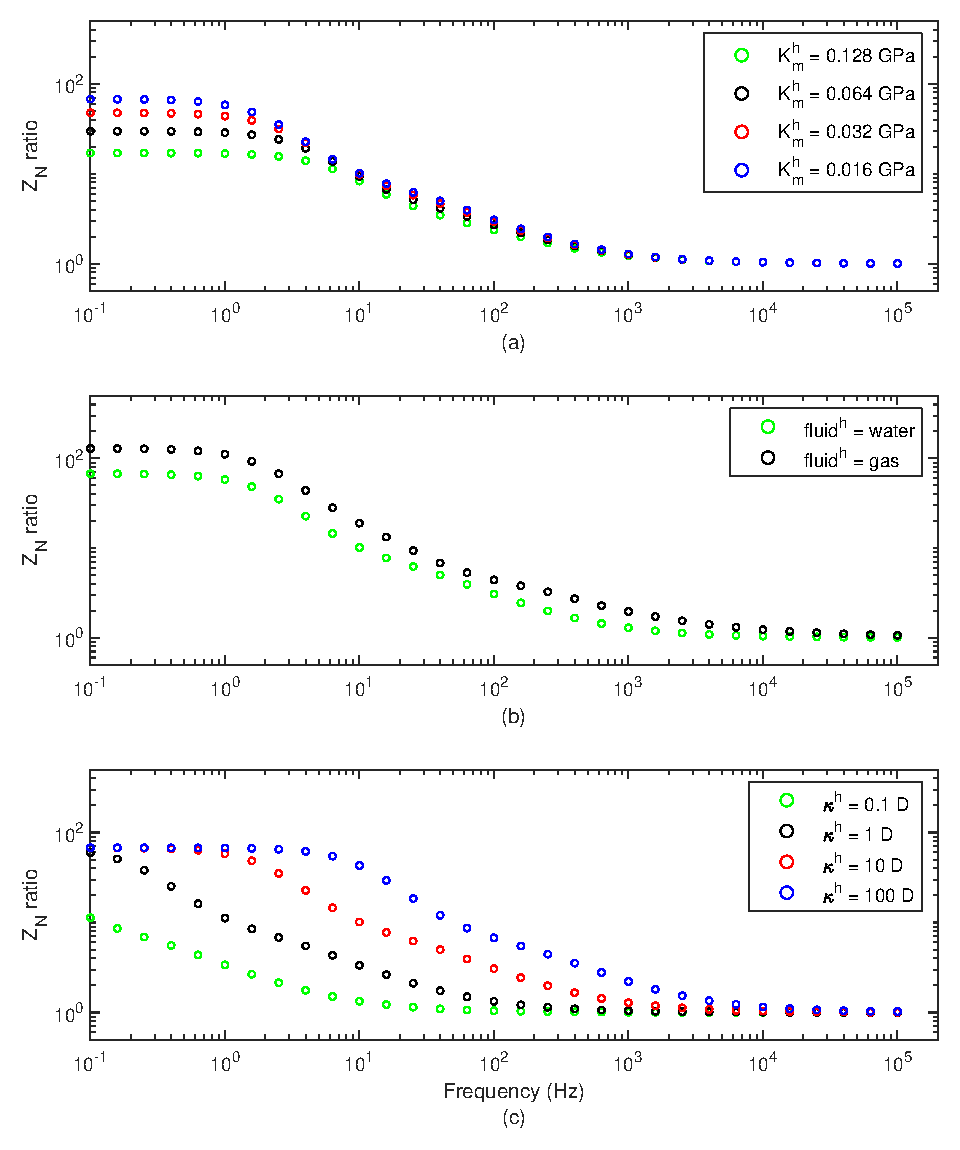
\includegraphics[ width=100mm, height=120mm]{sensitivityZN_physical.eps}
\caption{Ratio of the primary fracture normal compliance to its undrained value ($Z_N\, \text{ratio}$) as a function of frequency obtained considering secondary fractures with different a) bulk moduli $K_m^h$, b) permeabilities $\kappa^h$ and  c) pore fluids $f^h$. 
}
\label{fig.6}
\end{figure}

 \begin{figure}[!ht]
\centering
        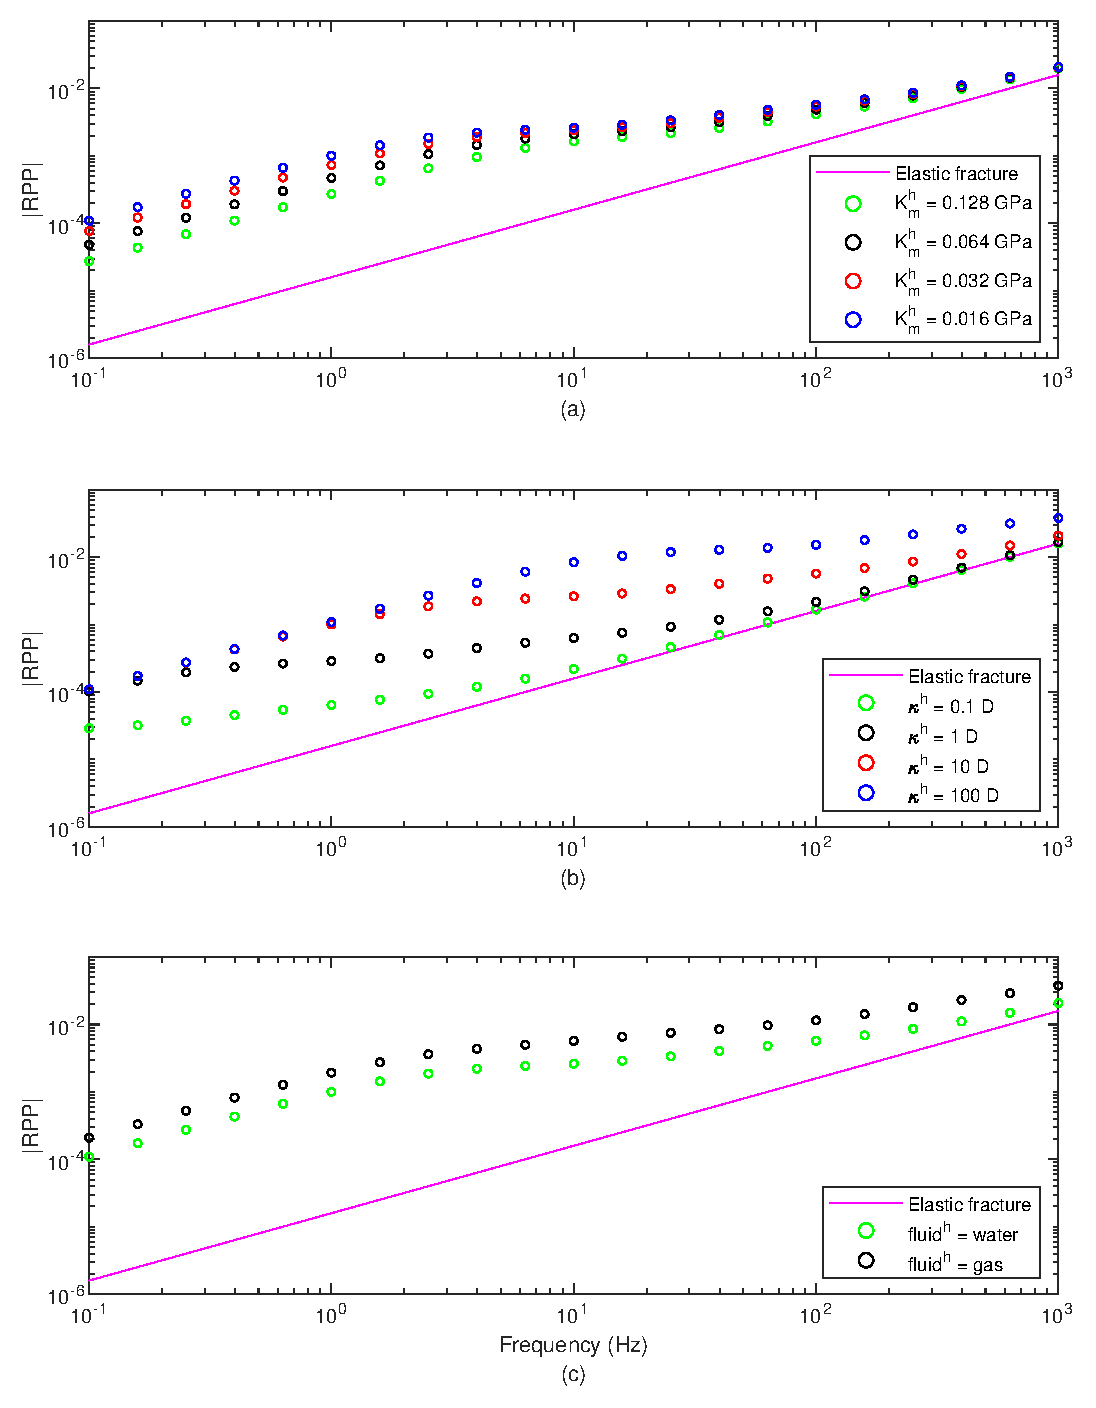
\includegraphics[ width=100mm, height=120mm]{sensitivityRPP_physical.eps}
\caption{ Absolute value of normal-incidence P-wave reflection coefficients as a function of frequency obtained considering different frequency-dependent P-wave moduli of the primary fracture. These moduli include the effect of FPD interactions with secondary fractures presenting different a) bulk moduli $K_m^h$, b) permeabilities $\kappa^h$ and  c) pore fluids $f^h$. For comparison, we also show the reflectivity curve of an isolated, that is, elastic primary fracture 
}
\label{fig.7}
\end{figure}

Figure \ref{fig.6}, presents the resulting $Z_N$ ratio as a function of frequency for the different physical properties of the secondary fractures.
These results also show that the presence of the secondary fractures  increases  the normal compliance of the primary fracture with respect to its unrelaxed value ($Z_N$ ratio of 1) for 
for frequencies associated with FPD prevailing in regimes
other than the unrelaxed one. 
In particular, the relaxed $Z_N$ ratio shows sensitivity to changes in bulk modulus $K_m^h$ (Figure \ref{fig.6}a) and in the pore fluid $f^h$ (Figure \ref{fig.6}c) of the secondary fractures. In fact, Figure \ref{fig.6}a shows that the relaxed $Z_N$ ratio increases close to 3-fold, from 15.9 to 43.5, which corresponds to an 8-fold decrease in the bulk modulus $K_m^h$, from 0.064 GPa to 0.008 GPa. These results suggest that  more deformable secondary fractures can accommodate larger fluid volumes coming from the primary fracture because their pores can expand more readily since they are softer.
Similarly, Figure \ref{fig.6}c shows an increase of $\sim$ 3.5-fold in the relaxed $Z_N$ ratio, from 43.5 to 150.1, when changing the saturating pore fluid from water to gas. This increase is the result of the higher compressibility of gas compared to that of water, which induces a higher pressure gradient for FPD to take place with the primary fracture. This, in turn, displaces larger fluid volumes from the primary fracture, which, consequently, generates a larger increase of its normal compliance.
On the other hand, the relaxed $Z_N$ ratio is insensitive to variations in the permeability of the secondary fractures (Figure \ref{fig.6}b). That is, for all tested permeabilities $\kappa^h$, the relaxed $Z_N$ ratio remains unchanged. The only effect that permeability has is on the characteristic transition frequency of the primary fracture compliance as described below.

Regarding the sensitivity of the characteristic transition frequency $f_c$ of the normal compliance of the primary fracture, our results show that $f_c$ increases from $\sim$ 5.6 Hz to $\sim$ 15.8 Hz as the bulk moduli $K_m^h$ increases. Similarly, we observe that $f_c$ increases from $\sim$ 1.4 Hz to $\sim$  5.6 Hz as the permeability $\kappa^h$ increases. Finally, $f_c$ decreases from $\sim$ 5.6 Hz to $\sim$ 2.8 Hz when the saturating fluid $f^h$ changes from water to gas.

Figure \ref{fig.7} shows that the increase of the primary fracture normal compliance due to FPD effects with the secondary fractures also produces an increase of its PP reflectivity with regard to the its elastic counterpart. We observe that, at sufficiently low frequencies there is a maximum increase of the primary fracture reflectivity as a consequence of FPD with the secondary fractures prevailing in the relaxed regime. Specifically, our results show that the highest increase of reflectivity is close to 1.5-orders-of-magnitude in this regime is associated with gas-saturated secondary fractures (Figure \ref{fig.7}c). Similary, the second highest reflectivity increase of $\sim$ 44-fold is associated with the softest secondary fractures ($K_m^h$ = 0.008 GPa in Figure \ref{fig.7}a) and for any of the tested permeabilities of the secondary fractures (Figure \ref{fig.7}b). This lack of sensitivity of the primary fracture reflectivity associated to changes in the permeability of the secondary fractures is consistent with the corresponding results for its compliance (Figure \ref{fig.6}b).  


\subsection{Summary of sensitivity analyses}
In this subsection we provide a general analysis regarding the effect that the geometrical and physical properties have on the normal compliance of the primary fracture at its relaxed state and on its characteristic transition frequencies $f_c$. To this end, Figure \ref{fig.8} presents the $Z_N$ ratio of the primary fracture associated with its relaxed state  (relaxed $Z_N$ ratio) versus the transition frequency $f_c$ of its normal compliance
for every of the previously tested properties of the secondary fractures. We further remark that, the relaxed $Z_N$ ratio reflects the maximum increase that the normal fracture compliance can attain with respect to its unrelaxed value for a given set of secondary fracture parameters (Figures \ref{fig.4} and  \ref{fig.6}).

 \begin{figure}[!ht]
\centering
        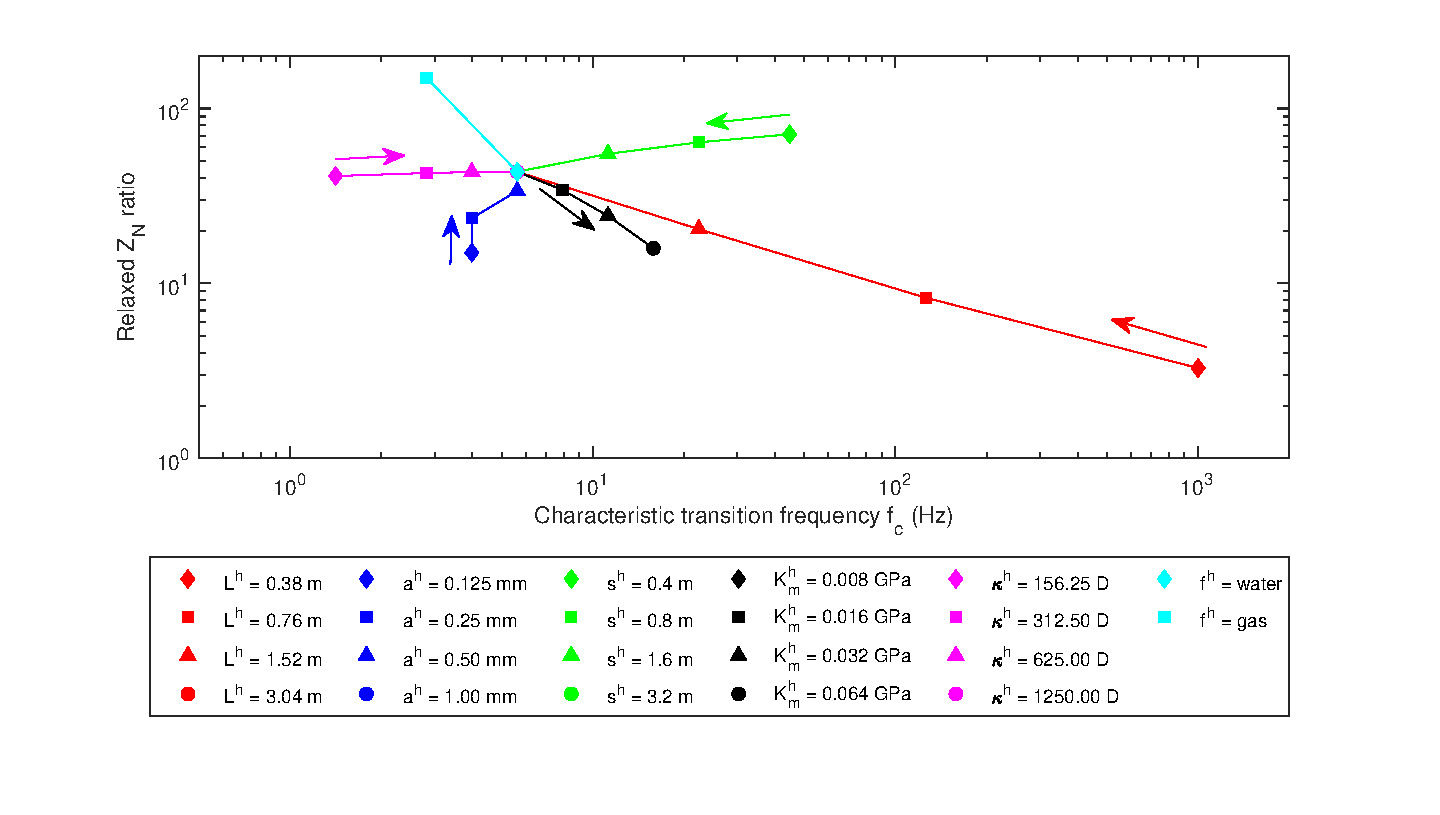
\includegraphics[ width=160mm, height=90mm]{sensitivity_summaryv2.eps}
\caption{ Relaxed $Z_N$ ratio of the primary fracture versus the characteristic transition frequency $f_c$ of its normal compliance for the considered properties of the secondary fractures ( \ref{fig.4} and \ref{fig.6}). The arrows point towards the direction, in which the properties of the secondary fractures increase in magnitude.
}
\label{fig.8}
\end{figure}

The results show that, overall, the relaxed $Z_N$ ratio is  most sensitive to changes in the length $L^h$ of the secondary fractures, with an increase of $\sim$ 13-fold, from  3.3 to 43.5, for an 8-fold increase of the length $L^h$.  This is followed by the the impact of changing the saturating pore fluid of the secondary fractures from water to gas, which produces an increase of the primary fracture relaxed $Z_N$ ratio of $\sim$ 3.5-folds, from 43.5 to 150.1.
Next, the changes in the bulk moduli $K_m^h$  and  in the aperture $a^h$  of the secondary fractures have similar impacts on the sensitivity of the relaxed  $Z_N$ ratio. This is, an 8-fold decrease in the bulk modulus and a similar increase in the aperture generate close to 3-fold increase in the corresponding relaxed $Z_N$ ratio, from $\sim$ 16 to 43.5,  respectively. 
The spacing $s^h$ of the secondary fractures has a much lower impact than the aforementioned properties on the sensitivity of the relaxed $Z_N$ ratio, where an 8-fold decrease of spacing  produces roughly a doubling of the the relaxed $Z_N$ ratio, from 43.5 to 71.2. 
Finally, as previously stated, changes in  the permeability $\kappa^h$ of the secondary fractures do not have any impact on the relaxed $Z_N$ ratio.

Changes in permeability of the secondary fractures affect the transition frequency $f_c$ of the primary fracture normal compliance. Higher permeabilities increase the transition frequency of the primary fracture normal compliance  in agreement with Equations \ref{Eq.3} and \ref{Eq.5}. Our results also show  a similar direct relationship of $f_c$ with the bulk modulus $K_m^h$ of the secondary fractures.
Conversely, we observe an inverse relationship of $f_c$  with the length $L^h$  and spacing $s^h$ of the secondary fractures. Indeed, it is possible to verify that $f_c$ decreases linearly with the inverse of the length to the power of 2.5 ($(L^h)^{-2.5}$) and as well as with the inverse of the spacing ($(s^h)^{-1}$), respectively. 
These results are consistent with Equation \ref{Eq.5}, which predicts an inverse proportionality between the transition frequency and the size of the characteristic heterogeneity of the secondary fractures, although to the power of two  ($(l_h)^{-2.0}$).  Next, $f_c$  presents a monotonically non-decreasing behavior with the increase of the aperture $a^h$ of the secondary fractures. Finally, we observe that gas-saturated secondary fractures induce a lower transition frequency $f_c$ compared to the water-saturated case. This is the direct consequence of the lower viscosity of gas compared to that of water (Equations \ref{Eq.3} and \ref{Eq.5}). 

\section{Discussion}

\subsection{Effect of correlated properties of the secondary fractures}
We have tested the sensitivity of the compliance and reflectivity of the primary fracture to variations in several properties of the secondary fractures, where the property of interest was gradually modified, while all
other properties were kept constant. In contrast to this analysis, we shall now assume that the properties of the secondary fractures are not independent but directly or indirectly correlated to their length, which is consistent with much of the available evidence \cite<e.g.,>{Hatton1994, Renshaw1995, Bonnet2001, Morris2017}.

Following this evidence, we use a power law  to relate the aperture $a^h$ to the length $L^h$ of the secondary fractures \cite<e.g.,>{Hatton1994}: $a^h = c_1 \, (L^h) ^{d_1}$, where $c_1$ = $10^{-3.4}$, $d_1$ = 1.05, respectively

We associate the permeability $\kappa^h$ of the secondary fractures to their hydraulic aperture $H^h$ through \cite{Zimmerman1996,Jaeger2009}: $\kappa^h=(H^h)^2/12$, where the hydraulic aperture is related to the arithmetic mean aperture of the secondary fractures as \cite{Renshaw1995, Jaeger2009}: $(H^h)^3=(a^h)^3 ( 1 + r^2)^{-1.5}$. Here we assume that the  previously estimated aperture $a^h$ is the arithmetic mean aperture of the secondary fractures and $r$ is the ratio between the corresponding standard deviation and the mean aperture, which we assume to be equal to 11. This value is on the same order to the one corresponding to natural fractures with high roughness values  \cite{Renshaw1995}.

It is also possible to relate the bulk $K_m^h$ and shear $\mu^h$ moduli of the secondary fractures to their drained normal $Z_N^h$ and tangential $Z_T^h$ compliances \cite{Nakagawa2007,Rubino2014}: $\mu^h = a^h/Z_T^h$ and $K_m^h =a^h/Z_N^h -4 \, a^h/(3\,Z_N^h)$, where the normal compliance of the secondary fractures can be further related to their length by a power law relationship  $Z_N^h = c_2 \, (L^h) ^{d_2}$, with $c_2$ = $10^{-10.7}$ and $d_2$ =0.77, respectively. This curve follows the trend of the data presented in \citeA{Barbosa2019}. Notice that the relationships for estimating the aperture and permeability of the secondary fractures show a monotonically increasing trend with respect to their length and aperture, respectively. 
%The relationships to estimate the respective shear and bulk moduli have a similar behavior  with respect to the ratio  of the aperture to the tangential and drained normal compliance. Consequently, the moduli are related to the aperture and the compliances in an opposing fashion.

Table \ref{table.3} summarizes the geometrical and physical properties for three different secondary fracture lengths: 0.7 m, 1.5 m and 2.9. Other properties are assumed to be the same for all cases and correspond to those listed in Table \ref{table.1} except the spacing of the secondary fractures, for which we consider a value of 1.6 m.  As expected, the estimated apertures and permeabilities of the secondary fractures increase with their length. A similar behavior is observed for the bulk and shear moduli, but, their increase correlates with the ratio of the aperture to the respective tangential and drained normal compliance.  For reference,  Table \ref{table.3} also presents the estimated normal and tangential compliance of the secondary fractures, which show an increasing compliant behavior with increasing length. Besides, we assume that both the main and secondary fractures are water saturated (Table \ref{table.2}).


\begin{table}[!ht]
  \caption{ Properties of the secondary fractures correlated to their length }
\begin{center}
  \begin{tabular}{ | l c  c  c | }
    \hline
    Property  & \multicolumn{3}{c |}{Secondary fracture ($h$)} \\ 
    \hline
    Length $L$ (m) & 0.7 & 1.5 & 2.9  \\
    Aperture $a$ (m) & 3.e-4 & 6.e-4 & 1.2e-3\\
    Permeability $\kappa$ (D) & 51.9 & 257.0 & 1026.1\\
    Frame bulk modulus $K_m$ (GPa)  & 0.010& 0.012 & 0.014 \\ 
    Frame shear modulus $\mu$ (GPa) & 0.006 & 0.008 & 0.009\\
    Drained normal compliance $Z_N$ (m/Pa)  & 1.5e.-11 & 2.7e-11 & 4.5e-11 \\
    Tangential compliance $Z_T$ (m/Pa) & 4.3e-11 & 7.8e-11 & 1.3e-10 \\    
    \hline
  \end{tabular}
  \label{table.3}
\end{center}
\end{table}

Figure \ref{fig.9} shows the impact that the three different sets of properties of the secondary fractures (Table \ref{table.3}) have on the  primary fracture normal compliance (Figure \ref{fig.9}a) and on the corresponding PP reflectivity  at normal incidence (Figure \ref{fig.9}a) as a function of frequency. Regarding effects on the primary fracture compliance, Figure \ref{fig.9}a shows that the relaxed $Z_N$ ratio takes increasingly higher values of 7.2, 19.7 and 51.6  as the length $L^h$ of the secondary fractures increases. This behavior suggest that the length of the secondary fractures controls the FPD interactions with the primary fracture. That is, longer secondary fractures generate higher pressure gradients and provide greater pore volumes that permit the drainage of higher volumes of pore fluid from the primary fracture. Figure \ref{fig.9}a  also shows that the characteristic transition frequency $f_c$ has the same value of 11.2 Hz for the three considered cases. 
This result implies that the tendency of progressively shorter fractures to increase  $f_c$ (Figure \ref{fig.4}a) is counterbalanced by the opposite effect that decreasing permeabilities have on $f_c$. We also remark that the relaxed $Z_N$ ratio of 51.6 induced by the longest secondary fractures (2.9 m) is higher than the one obtained in the sensitivity analyses for a secondary fracture length of 3.04 m, for which, the associated relaxed $Z_N$ ratio is 43.5. This higher relaxed $Z_N$ ratio is a consequence of the narrower spacing of the secondary fractures, 1.6 m instead of 3.2 m, which also has an influence in the characteristic transition frequency $f_c$, increasing its magnitude (Figures \ref{fig.4}c and \ref{fig.8}).

Figure \ref{fig.9}b shows that the absolute value of PP reflectivity at normal incidence of the primary fracture increases with increasing length $L^h$ of the secondary fractures compared to its elastic values, for frequencies corresponding to FPD regimes other than the unrelaxed one. This reflectivity behavior is produced by the softening of the normal compliance of the primary fractures that occurs as the secondary fractures lengthen (Figure \ref{fig.9}a).
Correspondingly, the maximum increase of  the primary fracture reflectivity of $\sim$ 50-fold is associated with the longest secondary fracture (2.9 m) for frequencies in the relaxed FPD regime. 


 \begin{figure}[!ht]
\centering
        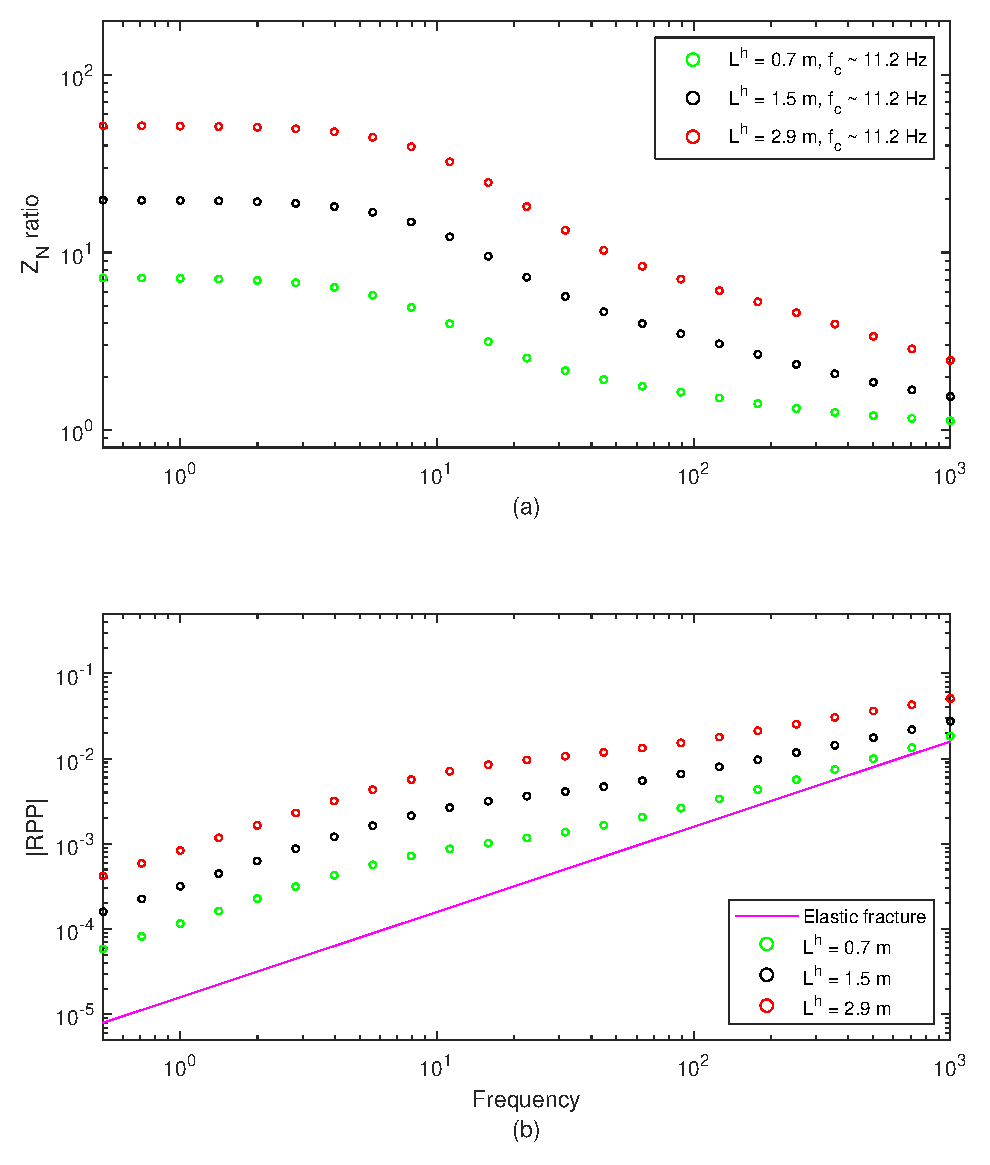
\includegraphics[ width=100mm, height=85mm]{linkedProperties.eps}
\caption{a) Ratio of the primary fracture normal compliance to its undrained value ($Z_N$ ratio) as a function of frequency considering secondary fractures presenting different properties correlated to their lengths $L^h$ (Table \ref{table.3}). b) Absolute value of normal-incidence P-wave reflection coefficient as a function of frequency considering different frequency-dependent P-wave moduli of the primary fracture. These moduli include the FPD effects with secondary fractures presenting the same properties as in (a).
}
\label{fig.9}
\end{figure}


\section{Conclusions}
We have investigated FPD effects between a large macroscopic primary fracture and secondary vertical fractures of mesoscopic scale induced by a P-wave  impinging normally onto the plane of the primary fracture. We have performed a sensitivity analysis of the primary fracture compliance and normal-incidence PP reflectivity with regard to variations of different geometrical and physical properties of the secondary fractures. Our results show that FPD interactions between the main and secondary fractures in the relaxed and transitional regimes produce an increase of the normal compliance and normal-incidence PP reflectivity of the primary fracture. Of the tested parameters, variations in the length of the secondary fractures produce the largest changes in the compliance of the primary fracture. The longest secondary fractures promote  $\sim$  43.5-fold increase of the normal compliance of the primary fracture from its undrained state, which leads to an increase of $\sim$ 44-fold of the primary fracture reflectivity. Our results also show that the characteristic transition frequency of the primary fracture compliance decreases with increasing length of the secondary fractures. More permeable and  more closely spaced secondary fractures counteract this tendency.  
Overall, our study suggest secondary mesoscopic fractures connected to a large primary fracture can induce FPD effects that substantially  enhance the seismic visibility of the primary fracture. 

However, we have considered and idealized but instructive canonical model of secondary fractures, which has allowed us to investigate the impact that the associated FPD has on the normal compliance and the PP reflectivity of a connected large primary fracture. To deepen our understanding of the influence of mesoscopic secondary fractures on the seismic behavior of macroscopic primary fractures due to FPD effects, it will be essential to explore more realistic networks of secondary fractures. Another important extension is to evaluate the reflectivity of such fracture systems for non-normal angles on incidence.

%Text here ===>>>

%  To add line numbers to lines in equations,
%  \begin{linenomath*}
%  \begin{equation}
%  \end{equation}
%  \end{linenomath*}



%% Enter Figures and Tables near as possible to where they are first mentioned:
%
% DO NOT USE \psfrag or \subfigure commands.
%
% Figure captions go below the figure.
% Table titles go above tables;  other caption information
%  should be placed in last line of the table, using
% \multicolumn2l{$^a$ This is a table note.}
%
%----------------
% EXAMPLE FIGURES
%
% \begin{figure}
% \includegraphics{example.png}
% \caption{caption}
% \end{figure}
%
% Giving latex a width will help it to scale the figure properly. A simple trick is to use \textwidth. Try this if large figures run off the side of the page.
% \begin{figure}
% \noindent\includegraphics[width=\textwidth]{anothersample.png}
%\caption{caption}
%\label{pngfiguresample}
%\end{figure}
%
%
% If you get an error about an unknown bounding box, try specifying the width and height of the figure with the natwidth and natheight options. This is common when trying to add a PDF figure without pdflatex.
% \begin{figure}
% \noindent\includegraphics[natwidth=800px,natheight=600px]{samplefigure.pdf}
%\caption{caption}
%\label{pdffiguresample}
%\end{figure}
%
%
% PDFLatex does not seem to be able to process EPS figures. You may want to try the epstopdf package.
%

%
% ---------------
% EXAMPLE TABLE
% Please do NOT include vertical lines in tables
% if the paper is accepted, Wiley will replace vertical lines with white space
% the CLS file modifies table padding and vertical lines may not display well
%

%% SIDEWAYS FIGURE and TABLE
% AGU prefers the use of {sidewaystable} over {landscapetable} as it causes fewer problems.
%
% \begin{sidewaysfigure}
% \includegraphics[width=20pc]{figsamp}
% \caption{caption here}
% \label{newfig}
% \end{sidewaysfigure}
%
%  \begin{sidewaystable}
%  \caption{Caption here}
% \label{tab:signif_gap_clos}
%  \begin{tabular}{ccc}
% one&two&three\\
% four&five&six
%  \end{tabular}
%  \end{sidewaystable}

%% If using numbered lines, please surround equations with \begin{linenomath*}...\end{linenomath*}
%\begin{linenomath*}
%\begin{equation}
%y|{f} \sim g(m, \sigma),
%\end{equation}
%\end{linenomath*}

%%% End of body of article

%%%%%%%%%%%%%%%%%%%%%%%%%%%%%%%%
%% Optional Appendix goes here
%
% The \appendix command resets counters and redefines section heads
%
% After typing \appendix
%
%\section{Here Is Appendix Title}
% will show
% A: Here Is Appendix Title
%
%\appendix
%\section{Here is a sample appendix}

%%%%%%%%%%%%%%%%%%%%%%%%%%%%%%%%%%%%%%%%%%%%%%%%%%%%%%%%%%%%%%%%
%
% Optional Glossary, Notation or Acronym section goes here:
%
%%%%%%%%%%%%%%
% Glossary is only allowed in Reviews of Geophysics
%  \begin{glossary}
%  \term{Term}
%   Term Definition here
%  \term{Term}
%   Term Definition here
%  \term{Term}
%   Term Definition here
%  \end{glossary}

%
%%%%%%%%%%%%%%
% Acronyms
%   \begin{acronyms}
%   \acro{Acronym}
%   Definition here
%   \acro{EMOS}
%   Ensemble model output statistics
%   \acro{ECMWF}
%   Centre for Medium-Range Weather Forecasts
%   \end{acronyms}

%
%%%%%%%%%%%%%%
% Notation
%   \begin{notation}
%   \notation{$a+b$} Notation Definition here
%   \notation{$e=mc^2$}
%   Equation in German-born physicist Albert Einstein's theory of special
%  relativity that showed that the increased relativistic mass ($m$) of a
%  body comes from the energy of motion of the body—that is, its kinetic
%  energy ($E$)—divided by the speed of light squared ($c^2$).
%   \end{notation}



%\section*{Open Research}

%%%%%%%%%%%%%%%%%%%%%%%%%%%%%%%%%%%%%%%%%%%%%%%

\acknowledgments
This work is supported by the grant 200020-178946 from the Swiss National Science Foundation. J. G. R. gratefully acknowledges the financial support received from CONICET (PIP 11220210100346CO).



%% ------------------------------------------------------------------------ %%
%% References and Citations

%%%%%%%%%%%%%%%%%%%%%%%%%%%%%%%%%%%%%%%%%%%%%%%
%
% \bibliography{<name of your .bib file>} don't specify the file extension
%
% don't specify bibliographystyle

% In the References section, cite the data/software described in the Availability Statement (this includes primary and processed data used for your research). For details on data/software citation as well as examples, see the Data & Software Citation section of the Data & Software for Authors guidance
% https://www.agu.org/Publish-with-AGU/Publish/Author-Resources/Data-and-Software-for-Authors#citation

%%%%%%%%%%%%%%%%%%%%%%%%%%%%%%%%%%%%%%%%%%%%%%%

\bibliography{reference}



%Reference citation instructions and examples:
%
% Please use ONLY \cite and \citeA for reference citations.
% \cite for parenthetical references
% ...as shown in recent studies (Simpson et al., 2019)
% \citeA for in-text citations
% ...Simpson et al. (2019) have shown...
%
%
%...as shown by \citeA{jskilby}.
%...as shown by \citeA{lewin76}, \citeA{carson86}, \citeA{bartoldy02}, and \citeA{rinaldi03}.
%...has been shown \cite{jskilbye}.
%...has been shown \cite{lewin76,carson86,bartoldy02,rinaldi03}.
%... \cite <i.e.>[]{lewin76,carson86,bartoldy02,rinaldi03}.
%...has been shown by \cite <e.g.,>[and others]{lewin76}.
%
% apacite uses < > for prenotes and [ ] for postnotes
% DO NOT use other cite commands (e.g., \citet, \citep, \citeyear, \citealp, etc.).
% \nocite is okay to use to add references from your Supporting Information
%



\end{document}



More Information and Advice:

%% ------------------------------------------------------------------------ %%
%
%  SECTION HEADS
%
%% ------------------------------------------------------------------------ %%

% Capitalize the first letter of each word (except for
% prepositions, conjunctions, and articles that are
% three or fewer letters).

% AGU follows standard outline style; therefore, there cannot be a section 1 without
% a section 2, or a section 2.3.1 without a section 2.3.2.
% Please make sure your section numbers are balanced.
% ---------------
% Level 1 head
%
% Use the \section{} command to identify level 1 heads;
% type the appropriate head wording between the curly
% brackets, as shown below.
%
%An example:
%\section{Level 1 Head: Introduction}
%
% ---------------
% Level 2 head
%
% Use the \subsection{} command to identify level 2 heads.
%An example:
%\subsection{Level 2 Head}
%
% ---------------
% Level 3 head
%
% Use the \subsubsection{} command to identify level 3 heads
%An example:
%\subsubsection{Level 3 Head}
%
%---------------
% Level 4 head
%
% Use the \subsubsubsection{} command to identify level 3 heads
% An example:
%\subsubsubsection{Level 4 Head} An example.
%
%% ------------------------------------------------------------------------ %%
%
%  IN-TEXT LISTS
%
%% ------------------------------------------------------------------------ %%
%
% Do not use bulleted lists; enumerated lists are okay.
% \begin{enumerate}
% \item
% \item
% \item
% \end{enumerate}
%
%% ------------------------------------------------------------------------ %%
%
%  EQUATIONS
%
%% ------------------------------------------------------------------------ %%

% Single-line equations are centered.
% Equation arrays will appear left-aligned.

Math coded inside display math mode \[ ...\]
 will not be numbered, e.g.,:
 \[ x^2=y^2 + z^2\]

 Math coded inside \begin{equation} and \end{equation} will
 be automatically numbered, e.g.,:
 \begin{equation}
 x^2=y^2 + z^2
 \end{equation}


% To create multiline equations, use the
% \begin{eqnarray} and \end{eqnarray} environment
% as demonstrated below.
\begin{eqnarray}
  x_{1} & = & (x - x_{0}) \cos \Theta \nonumber \\
        && + (y - y_{0}) \sin \Theta  \nonumber \\
  y_{1} & = & -(x - x_{0}) \sin \Theta \nonumber \\
        && + (y - y_{0}) \cos \Theta.
\end{eqnarray}

%If you don't want an equation number, use the star form:
%\begin{eqnarray*}...\end{eqnarray*}

% Break each line at a sign of operation
% (+, -, etc.) if possible, with the sign of operation
% on the new line.

% Indent second and subsequent lines to align with
% the first character following the equal sign on the
% first line.

% Use an \hspace{} command to insert horizontal space
% into your equation if necessary. Place an appropriate
% unit of measure between the curly braces, e.g.
% \hspace{1in}; you may have to experiment to achieve
% the correct amount of space.


%% ------------------------------------------------------------------------ %%
%
%  EQUATION NUMBERING: COUNTER
%
%% ------------------------------------------------------------------------ %%

% You may change equation numbering by resetting
% the equation counter or by explicitly numbering
% an equation.

% To explicitly number an equation, type \eqnum{}
% (with the desired number between the brackets)
% after the \begin{equation} or \begin{eqnarray}
% command.  The \eqnum{} command will affect only
% the equation it appears with; LaTeX will number
% any equations appearing later in the manuscript
% according to the equation counter.
%

% If you have a multiline equation that needs only
% one equation number, use a \nonumber command in
% front of the double backslashes (\\) as shown in
% the multiline equation above.

% If you are using line numbers, remember to surround
% equations with \begin{linenomath*}...\end{linenomath*}

%  To add line numbers to lines in equations:
%  \begin{linenomath*}
%  \begin{equation}
%  \end{equation}
%  \end{linenomath*}



